% -----------------------------------------------
% Template for ISMIR Papers
% 2018 version, based on previous ISMIR templates

% Requirements :
% * 6+n page length maximum
% * 4MB maximum file size
% * Copyright note must appear in the bottom left corner of first page
% * Clearer statement about citing own work in anonymized submission
% (see conference website for additional details)
% -----------------------------------------------

\documentclass{article}
\usepackage{ismir,amsmath,cite,url}
\usepackage{graphicx}
\usepackage{color}


% Title.
% ------
\title{GraphDitty: A Software Suite for Geometric Music Structure Visualization}

% Note: Please do NOT use \thanks or a \footnote in any of the author markup

% Single address
% To use with only one author or several with the same address
% ---------------
\oneauthor
 {Christopher J. Tralie}
 {Duke University Department of Mathematics}



\sloppy % please retain sloppy command for improved formatting
\graphicspath{{Figures/}}

\begin{document}

%
\maketitle
%

\section{Overview}\label{sec:introduction}

Music structure.

In this work, we present a techinque to create clean audio self-similarity matrices at the song level by fusing multiple features.  We also 


\begin{figure}
    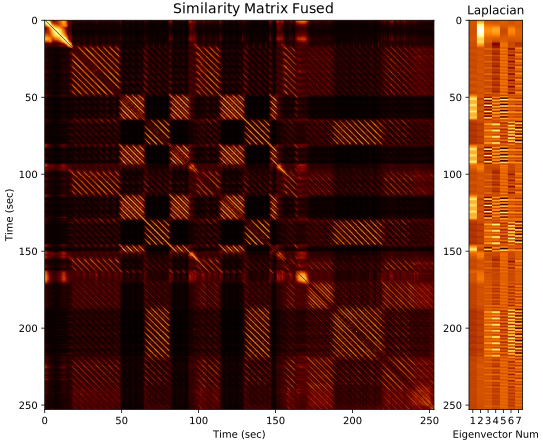
\includegraphics[width=\columnwidth]{SimilarityMatrix_Laplacian.pdf}
    \caption{Similarity matrix and Laplacian eigenvectors after applying similarity network fusion to stack-delayed Chroma and MFCC features.  The SSM and eigenvectors are noticeably cleaner than those with just raw chroma in Figure~\ref{fig:SSMChroma}.}
    \label{fig:SSMFused}
   \end{figure}

\begin{figure}
    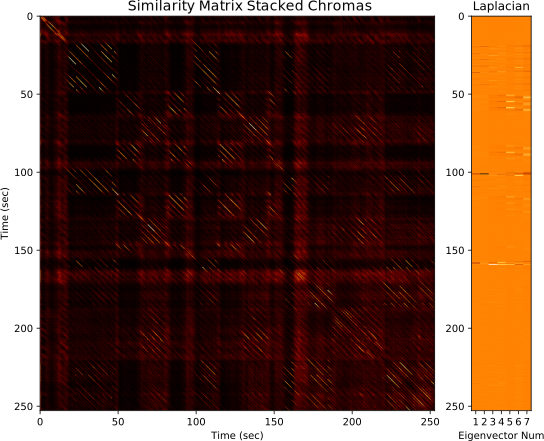
\includegraphics[width=\columnwidth]{SimilarityMatrix_Chroma.pdf}
    \caption{Similarity matrix using the cosine distance on stack-delayed Chroma features.}
    \label{fig:SSMChroma}
\end{figure}
   





\begin{figure}
 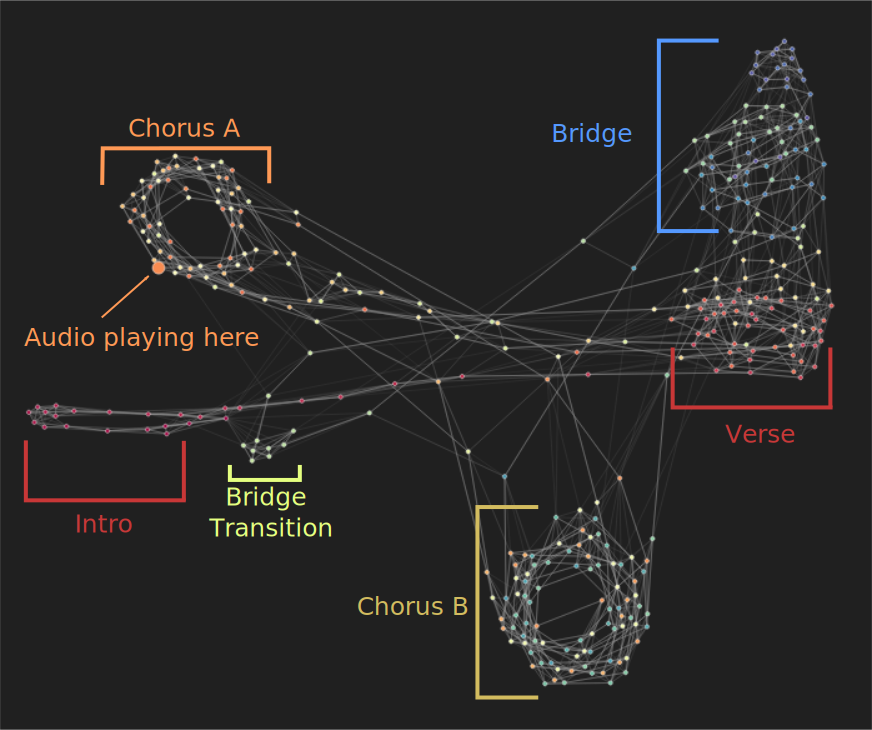
\includegraphics[width=\columnwidth]{ForceGraph.pdf}
 \caption{A dynamic weighted spring layout based on the weights in Figure~\ref{fig:SSMFused}, which is rendered with the help of d3.js \cite{bostock2012d3}.}
 \label{fig:example}
\end{figure}

Keypoints
*Code is clean with the help of numpy/scipy on the Python end and d3.js on the Javascript end, but it can be treated as a blackbox
*Not beat-synchronous
*Relies on similarity network fusion, which is simpler than diagonal promotion, etc
*Amenable to many different types of visualization
*Future work: exploring structure for audio cover song identification, similar to \cite{kinnaird2016aligned} on symbolic cover song identification

ROYGBIV figures

% For bibtex users:
\bibliography{main}

\cite{wang2012unsupervised, wang2014similarity,bendichgeometric,coifman2006diffusion,kinnaird2016aligned,mcfee2014analyzing,tralie2017cover,tralie2017Dissertation,bostock2012d3}

\end{document}
